% =====================================================================
%  DA-ZVAD — LIVING RESEARCH DOCUMENT
%  Elsevier CAS single-column format (cas-sc)
%  Maintained for supervisor review. Updated as findings arrive.
%
%  HOW TO MAINTAIN THIS DOCUMENT
%  -----------------------------
%  1. Add a row to the Revision History table (Document Status section)
%     every time you update something. This is how progress is tracked.
%  2. Replace \pending{...} markers with real content as results arrive.
%     Never delete a \pending marker without filling in the content.
%  3. New references go in references.bib; cite with \citep{} or \citet{}
%     (numbered style is active; both of those commands work).
%  4. Section order is fixed as agreed with the supervisor. Note that in
%     journal format the draft title and draft abstract live in the front
%     matter rather than as numbered sections.
%
%  BEFORE ACTUAL JOURNAL SUBMISSION
%  --------------------------------
%  Comment out the entire "Document Status" section (marked below) --
%  it exists for supervision tracking, not for reviewers.
% =====================================================================

\documentclass[a4paper,fleqn]{cas-sc}

% Numbered citation style, matching model1-num-names.bst shipped with the CAS
% bundle (and the convention of Pattern Recognition Letters / Neurocomputing).
% \citep gives [12]; \citet gives "Liu et al. [12]" -- both still work.
% To switch to author-year instead: use [authoryear,longnamesfirst] here and
% \bibliographystyle{cas-model2-names} at the end (that .bst must be present).
\usepackage[numbers,sort&compress]{natbib}

% cas-sc already provides: geometry, graphicx, hyperref, xcolor, natbib
% hooks, and enhanced enumerate/itemize. Do NOT load those again.
\usepackage{amsmath,amssymb}
\usepackage{booktabs}
\usepackage{tabularx}
\usepackage{algorithm}
\usepackage{algpseudocode}

% ---------- colours for status markers ----------
\definecolor{pendingcol}{HTML}{B03A2E}
\definecolor{donecol}{HTML}{1E8449}
\definecolor{notecol}{HTML}{6B6A63}

% ---------- status macros ----------
% \pending{what is still required} -- visible marker for unfinished content
\newcommand{\pending}[1]{{\sffamily\color{pendingcol}[\,PENDING: #1\,]}}
\newcommand{\done}{{\sffamily\bfseries\color{donecol}DONE}}
\newcommand{\inprog}{{\sffamily\bfseries\color{pendingcol}IN PROGRESS}}
\newcommand{\notstarted}{{\sffamily\bfseries\color{notecol}NOT STARTED}}
% \wnote{...} -- working note to supervisor / self (named to avoid any
% clash with class-provided note commands)
\newcommand{\wnote}[1]{{\color{notecol}\itshape #1}}

% ---------- table column types ----------
% cas-sc defines L, C and R itself, so ours use different letters.
% Z         : ragged-right stretchable column (tabularx)
% W{width}  : fixed-width ragged-right paragraph column
\newcolumntype{Z}{>{\raggedright\arraybackslash}X}
\newcolumntype{W}[1]{>{\raggedright\arraybackslash}p{#1}}

% =====================================================================
\begin{document}
\let\WriteBookmarks\relax
\def\floatpagepagefraction{1}
\def\textpagefraction{.001}

% ---------- running heads ----------
\shorttitle{Domain-adaptive zero-shot anomaly detection}
\shortauthors{P. K. Sarangi et~al.}

% ---------- title ----------
\title[mode = title]{Domain-Adaptive Zero-Shot Anomaly Detection Using
Vision-Language Models}

% ---------- authors ----------
\author[1]{Prakash Kumar Sarangi}[orcid=]
\cormark[1]
\ead{prakash_m251250cs@nitc.ac.in}
\credit{Conceptualization, Methodology, Software, Investigation, Writing --
original draft}

\affiliation[1]{organization={National Institute of Technology Calicut},
    addressline={Department of Computer Science and Engineering},
    city={Kozhikode},
    postcode={673601},
    state={Kerala},
    country={India}}

\author[1]{Pranesh Das}
\credit{Supervision, Conceptualization, Writing -- review and editing}

\author[1]{Raju Hazari}
\credit{Supervision, Writing -- review and editing}

\cortext[cor1]{Corresponding author}

% ---------- abstract ----------
\begin{abstract}
Video anomaly detection (VAD) models degrade when deployed in an environment
different from the one they were developed on. The established remedy is domain
adaptation (DA), and the overwhelming majority of DA research---as its own
surveys state explicitly---targets \emph{covariate shift}, the change in the
input distribution $p(x)$, while treating \emph{concept shift}, the change in
the conditional $p(y \mid x)$, as uncommon enough to set aside. We observe that
this assumption, reasonable for object classification, is invalid for anomaly
detection: normality in VAD is defined by deployment context rather than by
object identity, so the same visual input legitimately carries opposite labels
in different domains---a vehicle is normal on a road and anomalous on a
pedestrian walkway. Concept shift is therefore not a rare corner case in VAD but
its dominant form of domain shift. We further note that vision-language
foundation models such as CLIP already absorb much of the covariate shift that
classical DA was built to correct, leaving concept shift as the operative
problem. We propose DA-ZVAD, a fully training-free VAD pipeline in which every
model remains frozen and domain adaptation is performed exclusively through a
natural-language description of the deployment scene, injected at test time.
Because no parameters are updated anywhere in the pipeline, any change in
performance is attributable to the text alone, which makes the adaptation claim
directly measurable. We introduce an evaluation protocol that varies only this
description across four conditions---absent, generic, matched, and deliberately
mismatched---where the mismatched condition serves as a falsifying control. We
evaluate across industrial and surveillance domains. On MVTec~AD the frozen
scorer attains $88.5\%$ image-level AUROC with no training data, within four
points of a one-class baseline fitted on identical features. On the full
ShanghaiTech test set it attains $0.734$ frame-level AUROC with a matched
descriptor and $0.707$ with none. The sweep yields the predicted
signature---matched $0.734$ against mismatched $0.628$---but only once the
descriptor is injected into the normal ensemble alone. Appending it to both
ensembles draws the two prototypes together and reverses the effect, moving the
matched-minus-mismatched contrast from $-0.029$ to $+0.105$ and making an
accurate description the most damaging condition. The principal empirical
finding is that verbalized context is load-bearing but not robust: its measured
contribution is governed by the point of injection rather than by the wording,
and a fusion rule adopted without testing this inverts the conclusion drawn from
it. A replication on CUHK Avenue does not reproduce the effect, which we
attribute to that benchmark comprising a single scene.
\end{abstract}

% ---------- keywords ----------
\begin{keywords}
video anomaly detection \sep domain adaptation \sep concept shift \sep
vision-language models \sep training-free adaptation \sep explainability
\end{keywords}

\maketitle

% =====================================================================
% DOCUMENT STATUS  --  supervision tracking only.
% COMMENT OUT THIS ENTIRE SECTION BEFORE JOURNAL SUBMISSION.
% =====================================================================
\section*{Document Status}

\wnote{This document is maintained continuously for supervisor review. Content
not yet produced is marked inline with a \pending{} marker rather than left
blank or written speculatively. Alternative titles under consideration:
(i)~\emph{Language-Guided Domain Adaptation for Zero-Shot Video Anomaly
Detection}; (ii)~\emph{Concept Shift, Not Covariate Shift: Training-Free
Domain-Adaptive Video Anomaly Detection with Vision-Language Models}.}

\begin{table}[width=\linewidth,cols=4,pos=h]
\caption{Section-by-section completion status.}\label{tbl:status}
\begin{tabularx}{\linewidth}{@{}c l l Z@{}}
\toprule
\textbf{\S} & \textbf{Section} & \textbf{Status} & \textbf{Notes} \\
\midrule
--- & Title (front matter)             & \done       & May be refined \\
--- & Abstract (front matter)          & \inprog     & Results sentences await experiments \\
1   & Introduction                     & \done       & Motivation integrated; roadmap added \\
2   & Literature review                & \done       & 6 DA surveys, 12 VAD/VLM papers reviewed \\
3   & Observations and research gap    & \done       & Gap identified and grounded in the surveys \\
4   & Contribution points              & \done       & 5 contributions stated \\
5   & Problem formulation, objectives  & \done       & --- \\
6   & Proposed methodology             & \done       & Framework detailed; algorithms cited \\
7   & Results and analysis             & \inprog     & Image-domain baseline complete; video experiments await GPU runs \\
8   & Conclusion and discussion        & \notstarted & Awaits results \\
--- & References                       & \inprog     & Grows with the document \\
\bottomrule
\end{tabularx}
\end{table}

\begin{table}[width=\linewidth,cols=2,pos=h]
\caption{Revision history.}\label{tbl:revision}
\begin{tabularx}{\linewidth}{@{}l Z@{}}
\toprule
\textbf{Date} & \textbf{Update} \\
\midrule
07 August 2026 & Converted to Elsevier CAS single-column format. Sections drafted from
         the literature study; image-domain baseline reported; video
         experiments pending. \\
10 August 2026 & Supervisor revisions: Introduction and Literature Review separated
         into distinct sections, with motivation integrated into the
         Introduction; framework overview expanded with end-to-end data flow,
         scoring and smoothing equations, and design rationale; algorithms
         (ViT, CLIP, LLaVA, 4-bit quantisation, One-Class SVM) and evaluation
         metrics (AUROC, PR) now cited. \\
14 Aug 2026 & ShanghaiTech evaluated in full on GPU (107 clips, 20{,}449
         frames). Results~2--4 reported: temporal ablation, context sweep under
         two fusion rules, and component ablation with clip-level held-out
         partitions. Per-clip score normalisation added to the metrics protocol.
         Conclusion and limitations rewritten against measured outcomes.
         Results~5 (cross-domain) and~6 (explanations) remain outstanding. \\
15 Aug 2026 & Added a citation to \citet{wilkinghoff2026context}, who reach the
         same conclusion independently: what counts as normal depends on the
         setting. Observation~2 and Contribution~C1 now cite that paper and say
         what this work adds instead. We state the problem in domain-adaptation
         terms, we supply the context as a sentence rather than as extra sensor
         data, and we test whether the context changes anything. \\
18 Aug 2026 & Results corrected and extended. An analysis script had scored the
         cosine margin where the pipeline scores its softmax; the two rank
         identically but normalise per clip differently, so figures derived from
         that script were wrong. Component ablation recomputed: the semantic
         pathway alone is now the best configuration and the previously reported
         complementarity with a kinematic signal does not survive. The temporal
         window was extended and peaks at $w{=}31$, raising the headline from
         $0.706$ to $0.734$ and widening the context gap to $+0.105$. Six
         modifications are now recorded as failing to improve on the minimal
         configuration. A limitation on the metric's sensitivity to monotone
         rescaling was added. \\
18 Aug 2026 & Result~5 written: CUHK Avenue evaluated with the identical frozen
         configuration. Detection transfers ($0.706$ against $0.707$) but the
         context effect nearly vanishes ($+0.020$ against $+0.105$), with an
         accurate descriptor scoring below none. Attributed to Avenue being a
         single camera view where ShanghaiTech is thirteen, and marked as a
         conjecture with the control experiment that would settle it. Conclusion
         and limitations scoped accordingly. \\
19 Aug 2026 & Within-view control run. Evaluating the sweep inside a single
         ShanghaiTech camera view reduces the gap from $+0.105$ to $+0.034$,
         near the $+0.020$ measured on single-view Avenue, so the scene-diversity
         account of Result~5 is supported by measurement rather than by analogy
         between benchmarks. Qualifications recorded: the per-view estimates are
         noisy, three of nine are negative, and one view scores below chance
         throughout. \\
% ---- ADD NEW ROWS HERE (newest at the bottom) ----
\bottomrule
\end{tabularx}
\end{table}

\wnote{\textbf{Current status of results.} The MVTec~AD image-domain baseline
and the ShanghaiTech video-domain results (Results~1--4,
Section~\ref{sec:results}) are completed measurements on real data, obtained on
an NVIDIA A40; each carries a run manifest recording the code commit, hardware,
library versions and dataset counts that produced it. Results~5 (cross-domain
transfer) and~6 (explanations under domain shift) are outstanding and are marked
as such; the claims depending on them are not made. No number appears in this
document that has not been measured.}

% =====================================================================
% END OF DOCUMENT STATUS SECTION
% =====================================================================

% =====================================================================
\section{Introduction}
% =====================================================================

Anomaly detection identifies rare, unexpected events in images or video, and
underpins applications from industrial quality inspection to public-space
surveillance. The dominant formulation is one-class learning: a model of
``normal'' is estimated from a large corpus of normal samples, and deviations
from that model are flagged. Anomalies are by nature rare, diverse and difficult
to enumerate in advance, so learning what is \emph{normal} and treating
everything else as suspect is a natural and widely adopted design.

This formulation carries three practical costs. First, it requires a substantial
corpus of domain-specific normal data before the system can be used at all.
Second---and this is the concern that motivates the present work---the learned
notion of normality is bound to the environment in which it was estimated. A
change of camera, viewpoint, site or application invalidates the model, and
recovering performance requires fresh data collection and retraining. Third,
such systems emit a score without a justification, which limits their
usefulness to an operator who must decide what to do about an alert.

The second cost is conventionally addressed by \emph{domain adaptation} (DA), a
mature field with a large body of methods for transferring a model from a source
domain to a target domain. We observe, however, that the DA literature and the
anomaly detection setting are misaligned in a specific and consequential way.
Domain shift decomposes into several distinct types, and the DA literature
concentrates---by explicit and reasonable scoping decision---on
\emph{covariate shift}, the change in the input distribution. In anomaly
detection, normality is defined by the deployment context rather than by object
identity, so the same visual content can be normal in one environment and
anomalous in another. That is \emph{concept shift}, the shift type the
literature sets aside. Section~\ref{sec:gap} develops this argument in full.

A second development compounds the mismatch. Vision-language models trained at
web scale, such as CLIP \citep{radford2021clip}, recognise concepts specified
purely in natural language. The breadth of that training also makes them
substantially robust to the appearance variation that covariate-shift methods
were built to correct. If a foundation model already absorbs much of the
covariate shift, then what remains is precisely the shift the field excluded.

We therefore propose DA-ZVAD, a video anomaly detection pipeline in which every
model is frozen and adaptation to a new environment is performed solely by
supplying a natural-language description of the deployment scene at inference
time. Because no parameter is updated anywhere in the pipeline, any measured
change in behaviour is attributable to that description alone, which converts
the adaptation claim from an assertion into something directly measurable. We
accompany the method with an evaluation protocol that varies only the
description, including a deliberately incorrect description that acts as a
falsifying control.

The remainder of this document is organised as follows.
Section~\ref{sec:lit} reviews zero-shot anomaly detection, the classical domain
adaptation literature, adaptation in the language-model era, and prior domain
adaptation work specific to video anomaly detection.
Section~\ref{sec:gap} states the observations drawn from that literature and the
resulting research gap. Section~\ref{sec:contrib} lists the contributions,
Section~\ref{sec:problem} formalises the problem, and
Section~\ref{sec:method} describes the proposed framework.
Section~\ref{sec:results} reports results and analysis, and
Section~\ref{sec:conclusion} concludes.

% =====================================================================
\section{Literature Review}
\label{sec:lit}
% =====================================================================

\subsection{Zero-shot and training-free anomaly detection}
Vision-language models (VLMs) trained on web-scale image--text corpora, notably
CLIP \citep{radford2021clip}, permit classification of concepts specified purely
in natural language. WinCLIP \citep{jeong2023winclip} applied this to industrial
anomaly detection by scoring images against ensembles of ``normal'' and
``abnormal'' text prompts, requiring no task-specific training; AnomalyCLIP
\citep{zhou2024anomalyclip} learns object-agnostic prompts to improve
generalisation across categories. These are evaluated primarily on MVTec~AD
\citep{bergmann2019mvtec}, against trained baselines such as PatchCore
\citep{roth2022patchcore}.

In video, LAVAD \citep{zanella2024lavad} demonstrated fully training-free VAD by
captioning frames with a VLM, scoring caption sequences with a large language
model, and refining the result via cross-modal similarity. VERA
\citep{ye2025vera} keeps the VLM frozen and instead learns a set of verbal
\emph{guiding questions}, yielding explainable detection; notably, these
questions are optimised offline on source data, so the adaptation is not
performed at test time. AnyAnomaly \citep{anyanomaly2025} lets a user define the
anomaly of interest in text at inference time, and OVVAD \citep{wu2024ovvad}
addresses the open-vocabulary setting using a frozen CLIP encoder with a
lightweight trained temporal adapter.

\subsection{Domain adaptation: the classical view}
Domain adaptation is the subfield of transfer learning in which the task is
fixed and the data distribution changes. The literature is mature and well
surveyed. \citet{patel2015visual} review the shallow era---subspace alignment,
geodesic-flow interpolation between source and target subspaces, dictionary
learning, and projection of heterogeneous features into a shared latent space.
\citet{wang2018deep} provide the canonical deep taxonomy. They divide one-step
DA into three families. \emph{Discrepancy-based} methods minimise a measured
gap between the domains. \emph{Adversarial-based} methods train a feature
extractor to defeat a domain discriminator, so that the features it produces
carry no domain signal. \emph{Reconstruction-based} methods use reconstruction
as an auxiliary task that encourages invariance. Where source and target are too
far apart to bridge in one step, multi-step DA constructs intermediate domains
between them.

\citet{wilson2020survey} organise unsupervised DA by mechanism---domain-invariant
feature learning, domain mapping, normalisation statistics, ensembles,
target-discriminative methods---and decompose methods into interchangeable
components, alongside the generalisation bound that motivates divergence
minimisation. \citet{liu2022deep} survey modern unsupervised DA:
statistic alignment, adversarial learning, generative mapping, self-training and
self-supervision, applied across natural images, medical imaging, video,
language and time series. They also list open directions, among them
source-free adaptation, continuous and test-time adaptation, and adaptation in
the foundation-model era. \citet{singhal2023domain} consolidate the field,
stating the theoretical conditions under which DA is justified and categorising
settings by label-set relationship (closed-set, partial, open-set, universal).

\subsection{Domain adaptation beyond vision}
The mechanism of adaptation changes substantially in the language-model era.
\citet{fan2026llm} review large language model adaptation for geotechnical
engineering. They describe four strategies forming ``a continuum balancing cost,
complexity, and performance'': \emph{prompt engineering},
\emph{retrieval-augmented generation}, \emph{domain-adaptive pretraining} and
\emph{fine-tuning}. The two ends of that continuum matter here. Prompt
engineering is the cheapest and most immediate, but ``often lacks depth and
robustness''; fine-tuning gives the highest task precision at the highest cost
in compute and labels.
The relevant structural observation is that in this paradigm the model may remain
unchanged while the \emph{input context} carries the adaptation---a category
absent from the visual DA taxonomies above, which predate foundation models.

\subsection{Domain adaptation within video anomaly detection}
Work applying DA specifically to VAD falls into three groups, distinguished by
what the target domain costs. \emph{Learned adaptation} requires target data and
a training run: Ada-VAD \citep{adavad2024} pretrains a domain-invariant predictor
with synthesised abnormal samples and then adapts adversarially to a few target
frames. \emph{Meta-learned scene adaptation} reduces but does not remove that
cost: \citet{lu2020fewshot} meta-train across many scenes so that a
future-frame-prediction model adapts to an unseen scene from a handful of frames.
\emph{Zero-shot cross-domain} methods remove the target-time cost entirely: zxVAD
\citep{aich2023zxvad} performs cross-domain VAD without any target adaptation,
contrasting normal features against pseudo-anomalies synthesised by an untrained
network.

Two properties are common to all three. First, each still trains a model on
source data, so the notion of normality is fixed by source visual statistics.
Second, and decisively for the present work, none provides a channel through
which an operator can \emph{state} what normality means in the target
environment; adaptation is mediated entirely by pixels and parameters, never by
language.

% =====================================================================
\section{Observations from Literature and Research Gap}
\label{sec:gap}
% =====================================================================

\subsection{Observation 1: the field targets covariate shift by design}
A domain is a joint distribution $P(x,y) = P(y\mid x)\,P(x)$, and shift may occur
in any factor. Following the taxonomy of \citet{kouw2018introduction} as
presented by \citet{liu2022deep}, four types are distinguished, summarised in
Table~\ref{tbl:shifts}.

\begin{table}[width=\linewidth,cols=3,pos=h]
\caption{The four types of domain shift.}\label{tbl:shifts}
\begin{tabularx}{\linewidth}{@{}l W{2.6cm} Z@{}}
\toprule
\textbf{Shift type} & \textbf{Factor} & \textbf{Standard example} \\
\midrule
Covariate shift        & $p(x)$       & Same objects under a different camera, lighting, or weather \\
Conditional shift      & $p(x\mid y)$ & A class appears differently across domains \\
Label / target shift   & $p(y)$       & Class proportions differ between domains \\
\textbf{Concept shift} & $p(y\mid x)$ & \textbf{The same input carries a different label} (a tomato classified as a vegetable in one country and a fruit in another) \\
\bottomrule
\end{tabularx}
\end{table}

\citet{liu2022deep} state their scope explicitly: concept shift ``is, however,
usually not a common problem in popular object classification or semantic
segmentation tasks. As such, this review mainly focuses on the covariate shift
alignment in UDA, as is most commonly studied,'' listing the remaining shifts as
directions for future research. Consistently, \citet{singhal2023domain} give
covariate shift---$P(Y_s\mid X_s) = Q(Y_t\mid X_t)$---as the first theoretical
condition under which DA is justified, which is to say that classical DA theory
\emph{assumes concept shift away}.

\subsection{Observation 2: anomaly detection is concept-shift dominated}
In anomaly detection, normality is a property of the deployment context rather
than of the object. Table~\ref{tbl:conceptshift} gives three cases in which the
visual content is unchanged while the correct label inverts with the domain.

\begin{table}[width=\linewidth,cols=4,pos=h]
\caption{Concept shift in video anomaly detection. The third case is an actual
anomaly class in the ShanghaiTech benchmark \citep{liu2018shanghaitech}.}
\label{tbl:conceptshift}
\begin{tabularx}{\linewidth}{@{}Z l l l@{}}
\toprule
\textbf{Input $x$} & \textbf{Domain A} & \textbf{Domain B} & \textbf{Shift} \\
\midrule
A person running    & park: normal   & bank vault: anomalous        & $p(y\mid x)$ \\
A person lying down & beach: normal  & factory aisle: anomalous     & $p(y\mid x)$ \\
A vehicle           & road: normal   & walkway: anomalous           & $p(y\mid x)$ \\
\bottomrule
\end{tabularx}
\end{table}

These are concept shift by definition. Methods that align $p(x)$ cannot address them. That family is
the dominant one across \citet{wang2018deep}, \citet{wilson2020survey} and
\citet{liu2022deep}, and it is the wrong instrument here: $p(x)$ may be identical
across the two domains while only the labelling function differs.

\citet{wilkinghoff2026context} reach the same conclusion independently. They
observe that ``a specific observation may be normal under one operating
condition, yet anomalous under another'', and argue that judging such an
observation against a single fixed notion of normality creates what they term
``structural ambiguity''. Abnormality, they conclude, should be assessed
conditionally.

We read that agreement as support for the premise rather than as competition
for it. Three things separate the two accounts. First, we state the problem in
the vocabulary of the domain-adaptation literature, which is what makes the
mismatch in Observation~1 visible: the shift anomaly detection exhibits is the
one that literature sets aside. Second, their context arrives through additional
sensing modalities, whereas ours arrives as a sentence written by an operator
and needs no extra instrumentation. Third, their paper is a position: it argues
for conditional assessment and lists open problems. This work supplies a
mechanism, and a protocol that can establish whether the supplied context does
anything at all.

\subsection{Observation 3: foundation models relocate the problem}
\citet{liu2022deep} pose the foundation-model question directly and answer it in
part: such models ``are robust to the covariate shift in many cases,'' but ``it
is challenging to alleviate the label shift, without access to target domain
data. In addition, the concept shift can also cause a problem, even though there
are sufficient training data.'' A frozen CLIP encoder has been exposed to an
enormous diversity of cameras, lighting conditions, and viewpoints, so much of
the covariate shift that classical DA was constructed to correct is already
absorbed. What remains is precisely the shift the literature set aside.

\subsection{Statement of the research gap}
\begin{enumerate}[G1.]
  \item \textbf{Concept shift dominates VAD but is unstudied as such.} The DA
        literature scopes it out as uncommon; in VAD it is the primary shift.
        That normality is context-dependent has recently been argued
        \citep{wilkinghoff2026context}, but not in the vocabulary that locates
        the mismatch: no existing work states VAD domain shift in the DA
        literature's own taxonomy, where the exclusion becomes visible.
  \item \textbf{No protocol measures language-mediated adaptation.} The standard
        DA protocol compares source-trained against target-adapted accuracy,
        which presupposes a training step. There is no established way to test
        whether a \emph{description} adapted anything.
  \item \textbf{Foundation-model-era DA is empirically under-characterised.}
        Identified as an open direction by \citet{liu2022deep}, with little
        empirical evidence on which shifts a frozen VLM absorbs unaided.
  \item \textbf{Explanation quality under domain shift is unexamined.} None of
        the six DA surveys addresses it; explainable VAD \citep{ye2025vera} is
        evaluated in-domain only.
\end{enumerate}

\wnote{Scope discipline: this work targets G1 and G2 as primary contributions,
with G3 and G4 as supporting evidence. It does not claim to solve concept shift,
nor to exceed the state of the art in detection accuracy.}

% =====================================================================
\section{Contribution Points}
\label{sec:contrib}
% =====================================================================

\begin{enumerate}[C1.]
  \item \textbf{Characterisation.} We formalise concept shift, rather than
        covariate shift, as the dominant form of domain shift in video anomaly
        detection, and show that this follows from the definition of normality in
        the task. That normality is context-dependent has been argued
        concurrently and independently \citep{wilkinghoff2026context}. What we
        add is its statement in the formal vocabulary of the domain-adaptation
        literature. That vocabulary locates the mismatch precisely: the shift
        anomaly detection exhibits is the one that literature excludes by
        explicit scoping decision. It also explains why $p(x)$-alignment methods
        are structurally unsuited to the task.

  \item \textbf{Mechanism.} We present DA-ZVAD, a fully training-free VAD
        pipeline in which every model is frozen and domain adaptation is
        performed solely by a natural-language description of the deployment
        scene supplied at test time. This transplants the lowest-cost strategy of
        the LLM adaptation continuum \citep{fan2026llm} into a vision task, and
        requires neither target-domain data nor gradient updates.

  \item \textbf{Evaluation protocol.} We introduce a four-condition context sweep
        (absent, generic, matched, mismatched) that isolates the contribution of
        the verbalised description while holding all else fixed. The
        \emph{mismatched} condition is a falsifying control: if supplying a
        wrong-domain description does not degrade performance, the adaptation
        claim is refuted.

  \item \textbf{Cross-domain empirical study.} We evaluate a single frozen
        pipeline across industrial and surveillance domains, providing evidence
        on which shifts a vision-language foundation model absorbs unaided and
        which it does not.

  \item \textbf{Explanation under shift.} We report the first examination of how
        generated natural-language explanations behave when the supplied domain
        context is incorrect.
\end{enumerate}

% =====================================================================
\section{Problem Formulation and Objectives}
\label{sec:problem}
% =====================================================================

\subsection{Formulation}
Let a domain $\mathcal{D}$ be a joint distribution $P(x,y)$ over inputs
$x \in \mathcal{X}$ (video frames or images) and labels $y \in \{0,1\}$, where
$y=1$ denotes anomalous. Let $\mathcal{D}_A$ and $\mathcal{D}_B$ be two
deployment domains. The concept-shift setting is characterised by
\begin{equation}
p_A(x) \approx p_B(x)
\qquad\text{while}\qquad
p_A(y \mid x) \neq p_B(y \mid x),
\label{eq:conceptshift}
\end{equation}
that is, visually comparable inputs receive different labels because the
definition of normality differs between the domains.

Classical unsupervised DA seeks a feature map $\phi$ minimising a divergence
$d\!\left(p_A(\phi(x)),\, p_B(\phi(x))\right)$. Under
Equation~\eqref{eq:conceptshift} this objective is uninformative, since the
marginals are already aligned; the quantity that differs is the labelling
function itself.

We therefore introduce an explicit domain descriptor $c \in \mathcal{C}$, a short
natural-language statement of what the deployment scene contains and what
constitutes normal behaviour within it. The anomaly score becomes
\begin{equation}
s(x \mid c) \;=\; f_\theta(x,\, c), \qquad \theta \ \text{fixed},
\label{eq:score}
\end{equation}
where $f_\theta$ is composed entirely of pre-trained, frozen models. Adaptation
from $\mathcal{D}_A$ to $\mathcal{D}_B$ consists of replacing $c_A$ with $c_B$;
no element of $\theta$ is updated, and no target-domain data is required.

Because $\theta$ is fixed by construction, any measured difference between
$s(x\mid c_A)$ and $s(x\mid c_B)$ is attributable to the descriptor alone. This
identifiability property is what makes the adaptation claim testable, and it is
not available to methods that update parameters.

\subsection{Setting}
In the vocabulary of the DA literature, the setting is: \emph{source-free} (no
source-domain data at adaptation time), \emph{test-time} (adaptation occurs at
inference), \emph{training-free} (no gradient updates anywhere),
\emph{concept-shift-oriented} (the targeted shift is in $p(y\mid x)$), and
\emph{language-mediated} (adaptation is carried by text).

\subsection{Objectives}
\begin{enumerate}[O1.]
  \item Formalise domain shift in VAD and establish concept shift as its dominant
        form.
  \item Design and implement a fully training-free detection pipeline in which
        domain context enters only as language.
  \item Devise and apply a protocol that isolates and measures the effect of the
        verbalised domain descriptor, including a falsifying control.
  \item Evaluate across industrial and surveillance domains, quantifying which
        shifts the frozen vision-language backbone absorbs unaided.
  \item Generate natural-language explanations for detected events and examine
        their behaviour under correct and incorrect domain context.
\end{enumerate}

% =====================================================================
\section{Proposed Methodology}
\label{sec:method}
% =====================================================================

\subsection{Framework overview}
DA-ZVAD is a four-stage inference pipeline in which every learned component is a
pre-trained model used with its weights frozen. Figure~\ref{fig:arch} shows the
architecture. This subsection describes the end-to-end data flow and the design
rationale; the individual modules are specified in Section~\ref{sec:modules} and
the complete procedure is given as Algorithm~\ref{alg:infer}.

\subsubsection{End-to-end data flow}
The system consumes a sequence of frames $X = \{x_1,\dots,x_T\}$ together with a
single natural-language domain descriptor $c$, and returns a per-frame anomaly
score together with a natural-language explanation for each detected event. Five
stages are executed in order.

\begin{enumerate}[Stage 1.]
  \item \textbf{Prompt construction.} Two prompt ensembles are instantiated from
        templates: a \emph{normal} ensemble $P^{+}$ and an \emph{abnormal}
        ensemble $P^{-}$. If the verbalised context module is active, the domain
        descriptor $c$ is injected into both ensembles, so that the textual
        definition of normality is specific to the deployment scene rather than
        generic. Ensembling several phrasings rather than using a single prompt
        follows the practice established for zero-shot anomaly detection by
        \citet{jeong2023winclip}.

  \item \textbf{Text encoding.} Each ensemble is encoded by the frozen text
        encoder and mean-pooled into a single unit-norm prototype vector,
        yielding $e^{+}$ and $e^{-}$. Because the descriptor enters only here,
        the entire influence of the domain context on detection is mediated by
        these two vectors.

  \item \textbf{Frame scoring.} Each frame is embedded by the frozen image
        encoder to give $v_t$. The anomaly score is the softmax probability that
        the frame matches the abnormal prototype rather than the normal one. It
        is computed over the two cosine similarities, scaled by the temperature
        $\lambda$ that the backbone learned during its own pre-training
        \citep{radford2021clip}:
        \begin{equation}
        s_t \;=\; \frac{\exp\!\left(\lambda \langle v_t, e^{-}\rangle\right)}
                       {\exp\!\left(\lambda \langle v_t, e^{+}\rangle\right)
                       +\exp\!\left(\lambda \langle v_t, e^{-}\rangle\right)}.
        \label{eq:framescore}
        \end{equation}
        No classifier is trained: the separation between the two text
        prototypes is what performs the classification.

  \item \textbf{Temporal aggregation.} The raw score sequence
        $s = (s_1,\dots,s_T)$ is smoothed by a centred moving average of width
        $w$,
        \begin{equation}
        \tilde{s}_t \;=\; \frac{1}{|\mathcal{W}_t|}
                          \sum_{k \in \mathcal{W}_t} s_k ,
        \qquad
        \mathcal{W}_t = \left[t - \lfloor w/2 \rfloor,\;
                              t + \lfloor w/2 \rfloor\right] \cap [1,T],
        \label{eq:smooth}
        \end{equation}
        which suppresses isolated single-frame excursions while preserving
        events that persist across several frames. The operator has no learnable
        parameters, so the temporal stage adds no training requirement.

  \item \textbf{Detection and explanation.} Frames with
        $\tilde{s}_t \ge \tau$ are flagged. Contiguous runs of flagged frames are
        grouped into events, and the single highest-scoring frame of each run is
        selected as that event's representative. Only these representative frames
        are passed to the multimodal language model, together with the same
        descriptor $c$, which produces the explanation. Explaining one frame per
        event rather than every flagged frame keeps the cost of the most
        expensive stage proportional to the number of events rather than to video
        length.
\end{enumerate}

\subsubsection{Design rationale}
Three properties of this arrangement are deliberate and worth stating explicitly.

\emph{Everything is frozen.} No gradient is computed anywhere in the pipeline.
This is not merely an efficiency choice: it is what makes the central claim
measurable. Since the parameters cannot change, a difference in output between
two runs that differ only in $c$ must be caused by $c$. Methods that update
weights cannot isolate the effect of a contextual input in this way.

\emph{The domain enters at exactly one point.} The descriptor is consumed in
Stage~1 (and again in Stage~5 for explanation), and nowhere else. Detection
therefore has a single, well-defined channel through which environment-specific
knowledge is supplied, which is what allows the context sweep of
Section~\ref{sec:sweep} to isolate its contribution.

\emph{The expensive stage is gated.} The visual encoder runs once per frame,
which is cheap and batchable; the language model runs once per detected event.
The pipeline therefore fits within roughly 7\,GB of accelerator memory, and its
cost does not scale with the length of quiet video.

\subsection{Module specifications}
\label{sec:modules}

% figure (not figure*): cas-sc is a single-column class, so a starred
% float would have nothing extra to span.
\begin{figure}[pos=h]
\centering
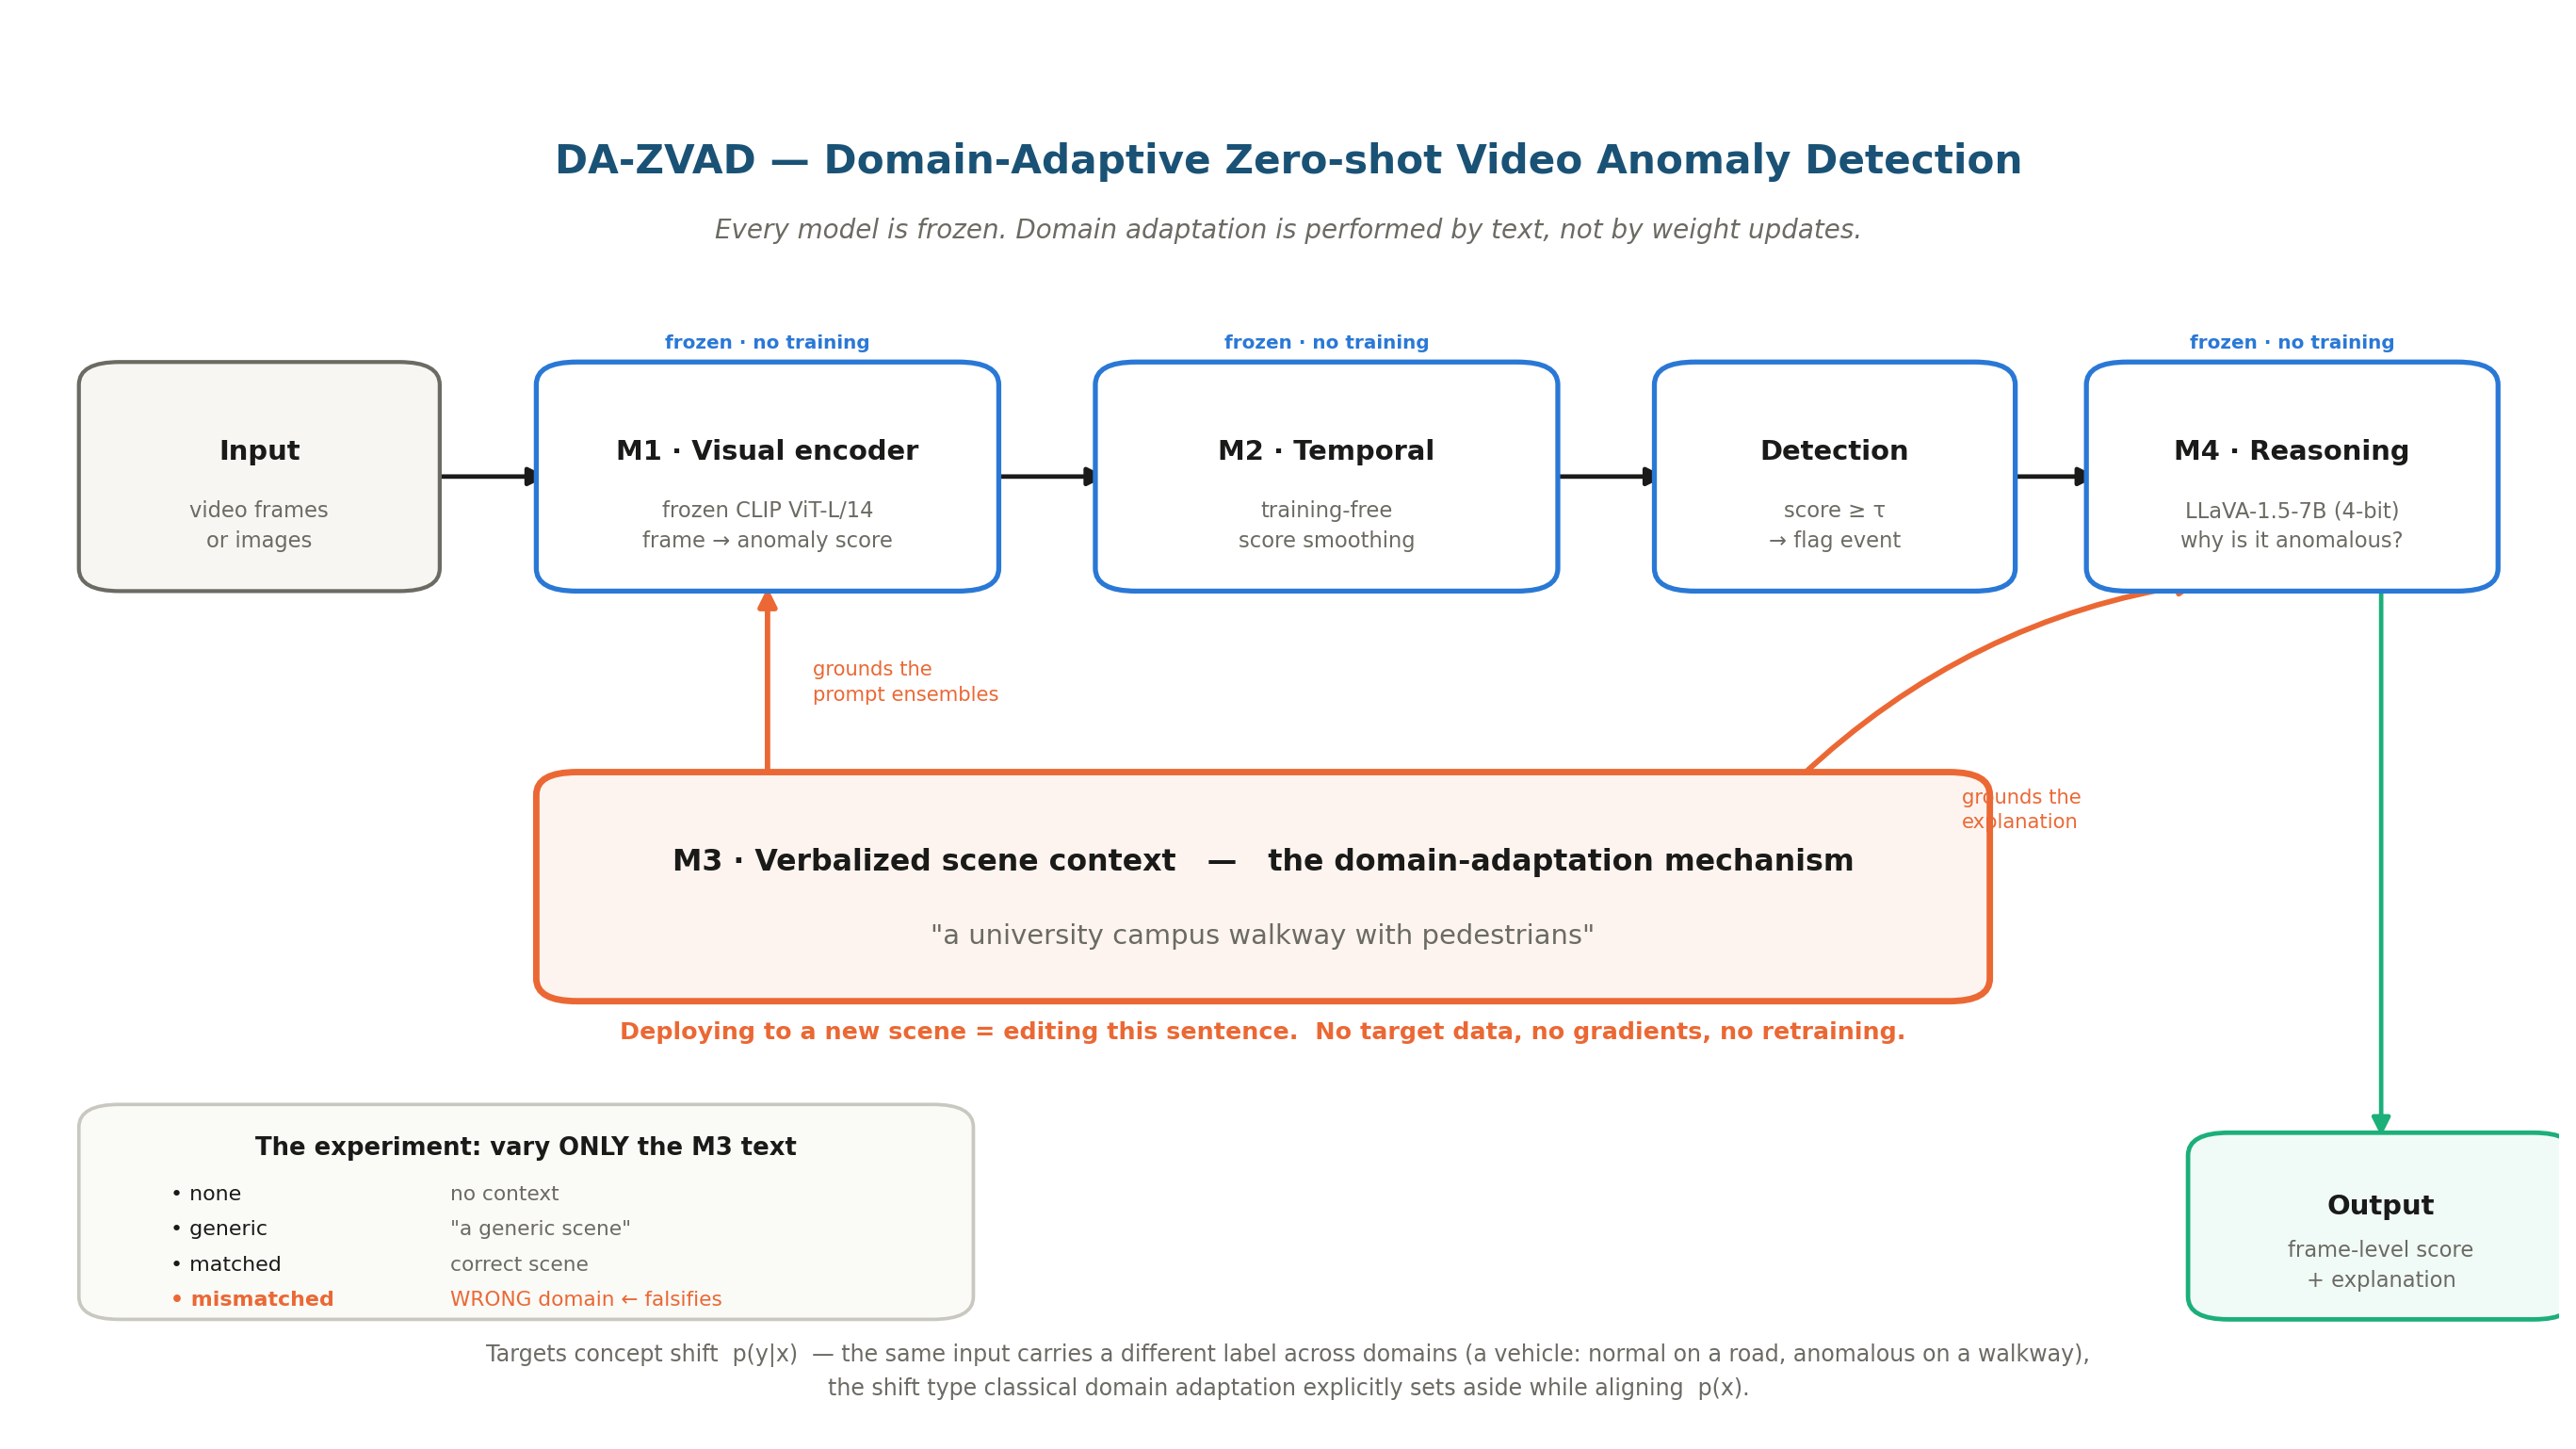
\includegraphics[width=\linewidth]{dazvad_architecture.png}
\caption{The DA-ZVAD framework. Every model is frozen; the verbalised scene
context (M3) is the sole adaptation mechanism, grounding both the prompt
ensembles used for scoring and the generated explanations.}
\label{fig:arch}
\end{figure}

\begin{description}
  \item[M1 --- Visual encoder.] A frozen CLIP ViT-L/14 encoder
  \citep{radford2021clip} embeds each frame. The backbone is a Vision
  Transformer \citep{dosovitskiy2021vit}, built on the transformer architecture
  of \citet{vaswani2017attention}. It partitions the frame into
  $14 \times 14$ patches and produces one unit-norm embedding, placed in the
  joint image--text space that CLIP learns by contrastive pre-training. Scoring
  follows Equation~\eqref{eq:framescore}. No training data is used; the
  language prior serves as the classifier.

  \item[M2 --- Temporal aggregation.] Per-frame scores are smoothed by the
  centred moving average of Equation~\eqref{eq:smooth} over a window of $w$
  frames. This suppresses isolated single-frame fluctuations while preserving
  multi-frame events, and introduces no learnable parameters. The window width
  $w$ is the only hyperparameter of this stage and is swept in
  Section~\ref{sec:results}.

  \item[M3 --- Verbalised domain context.] A short natural-language description
  of the deployment scene is injected into both prompt ensembles, grounding the
  notion of normality in the specific environment. This module is the adaptation
  mechanism of the framework. It is the vision-side counterpart of prompt-based
  adaptation as catalogued for language models by \citet{fan2026llm}, and
  differs from the verbalised learning of \citet{ye2025vera} in that the text is
  supplied at inference rather than optimised on source data beforehand.

  \item[M4 --- Reasoning and explanation.] For each detected event, a frozen
  multimodal large language model (LLaVA-1.5-7B \citep{liu2023llava}) receives
  the peak-scoring frame together with the domain descriptor and produces a
  natural-language explanation. The model is loaded under 4-bit
  \textsc{NormalFloat} quantisation \citep{dettmers2023qlora}, which reduces its
  memory footprint to roughly 5.5\,GB with negligible loss of generation
  quality. The prompt explicitly permits the model to report that nothing
  appears wrong, which limits ungrounded assertions.
\end{description}

The complete pipeline is designed to fit a single consumer GPU, using
approximately 7\,GB of VRAM. This is a deliberate contrast to multi-model
training-free pipelines such as that of \citet{zanella2024lavad}, which chains a
captioner, a large language model and a cross-modal refiner.

\subsection{Inference algorithm}
\begin{algorithm}[h]
\caption{DA-ZVAD inference for one sequence}
\label{alg:infer}
\begin{algorithmic}[1]
\Require frames $X = \{x_1,\dots,x_T\}$; domain descriptor $c$; window $w$;
         threshold $\tau$; frozen encoder $E$, frozen MLLM $G$
\Ensure per-frame scores $\tilde{s}$; event explanations $\mathcal{E}$
\State $(P^{+}, P^{-}) \gets \textproc{GroundPrompts}(c)$
       \Comment{M3: inject $c$ into prompt ensembles}
\State $e^{+} \gets \textproc{MeanPool}(E_{\text{text}}(P^{+}))$
\State $e^{-} \gets \textproc{MeanPool}(E_{\text{text}}(P^{-}))$
\For{$t = 1$ \textbf{to} $T$}
    \State $v_t \gets E_{\text{img}}(x_t)$ \Comment{M1: frozen visual embedding}
    \State $s_t \gets \textproc{Softmax}\!\left(\left[\langle v_t, e^{+}\rangle,\;
           \langle v_t, e^{-}\rangle\right]\cdot\lambda\right)_{2}$
           \Comment{$\lambda$: CLIP logit scale}
\EndFor
\State $\tilde{s} \gets \textproc{MovingAverage}(s, w)$ \Comment{M2}
\State $\mathcal{P} \gets \{t : \tilde{s}_t \ge \tau\}$
\State $\mathcal{V} \gets \textproc{PeakOfEachRun}(\mathcal{P}, \tilde{s})$
       \Comment{one explanation per event}
\ForAll{$t \in \mathcal{V}$}
    \State $\mathcal{E}[t] \gets G(x_t,\, c,\, \tilde{s}_t)$ \Comment{M4}
\EndFor
\State \Return $\tilde{s}, \mathcal{E}$
\end{algorithmic}
\end{algorithm}

\subsection{The context sweep protocol}
\label{sec:sweep}
To isolate the contribution of the domain descriptor, the pipeline is executed
repeatedly on identical data with every component fixed, varying only $c$ across
the four conditions of Table~\ref{tbl:variants}.

\begin{table}[width=\linewidth,cols=3,pos=h]
\caption{The four conditions of the context sweep. All models, frames,
thresholds and windows are held fixed; only the text differs.}
\label{tbl:variants}
\begin{tabularx}{\linewidth}{@{}l Z Z@{}}
\toprule
\textbf{Condition} & \textbf{Descriptor supplied} & \textbf{Purpose} \\
\midrule
none       & M3 disabled; prompt ensembles only & Lower reference \\
generic    & ``a generic scene''                & Controls for the mere presence of context \\
matched    & Correct description of the scene   & The proposed operating condition \\
mismatched & Description of the \emph{wrong} domain family (industrial text on surveillance data, and conversely) & \textbf{Falsifying control} \\
\bottomrule
\end{tabularx}
\end{table}

The predicted signature, if the adaptation claim holds, is
matched~$\gtrsim$~generic~$\gtrsim$~none, with mismatched performing measurably
\emph{worse}. The mismatched condition is essential: a method that ignores its
context entirely would show no difference across conditions, and a result of that
form would refute the claim rather than support it.

\subsection{Implementation}
The framework is implemented as a configuration-driven Python package in which
each module is independently switchable, so that the full ablation is produced by
configuration rather than by code modification. Experiments are cached and
resumable. The implementation has been verified end-to-end on synthetic data; the
measured results reported below are those obtained on real data.

Video experiments were run on a single NVIDIA A40 under PyTorch 2.3.1 with CUDA
12.1, using CLIP ViT-L/14 pretrained on LAION-2B. Each run records a manifest. It captures the
commit identifier of the code, the hardware, the library versions, the full
configuration, and the per-dataset sequence, frame and positive-label counts.
Every reported figure is therefore traceable to the state that produced it. Image embeddings are cached separately from scores: the visual encoder is
the only expensive stage and is independent of the prompts, the scoring rule and
the temporal window, so a single encoding pass supports the comparison of many
scoring hypotheses without re-encoding.

% =====================================================================
\section{Results and Analysis}
\label{sec:results}
% =====================================================================

\subsection{Datasets}
\begin{table}[width=\linewidth,cols=4,pos=h]
\caption{Datasets. The industrial/surveillance pairing provides the
concept-shift contrast: what constitutes normality differs maximally between
them.}\label{tbl:datasets}
\begin{tabularx}{\linewidth}{@{}l l Z l@{}}
\toprule
\textbf{Dataset} & \textbf{Domain} & \textbf{Content} & \textbf{Status} \\
\midrule
MVTec AD \citep{bergmann2019mvtec} & Industrial & 15 product categories, 1{,}725 test images, pixel-level masks & \done \\
ShanghaiTech \citep{liu2018shanghaitech} & Surveillance & Campus CCTV, 13 scenes, 107 test clips, 40{,}791 frames, frame-level ground truth & \done \\
CUHK Avenue \citep{lu2013avenue} & Surveillance & Outdoor campus walkway, single view, 21 test videos, 15{,}324 frames & \done \\
\bottomrule
\end{tabularx}
\end{table}

\subsection{Evaluation metrics}
Anomaly detection is a strongly class-imbalanced problem, in which accuracy is
uninformative: a detector that labels every frame normal attains high accuracy
while detecting nothing. We therefore adopt threshold-free and
imbalance-aware measures.

\begin{itemize}
  \item \textbf{AUROC} (primary). The area under the receiver operating
        characteristic curve \citep{fawcett2006roc, bradley1997auc}. It is
        threshold-free, and admits the equivalent probabilistic reading that it
        equals the probability that a randomly chosen anomalous sample receives
        a higher score than a randomly chosen normal one. It therefore measures
        the quality of the score \emph{ranking} rather than of any particular
        operating point, which is what makes results comparable across methods
        that calibrate their scores differently. Reported at image level for
        MVTec~AD and at frame level for video, following the convention of the
        respective benchmarks \citep{bergmann2019mvtec, liu2018shanghaitech}.

  \item \textbf{Micro- and macro-averaged AUROC.} Micro-averaging concatenates
        all frames across clips before computing a single curve, which weights
        long clips more heavily and is the usual convention on video benchmarks;
        macro-averaging computes AUROC per clip and averages, weighting clips
        equally. Divergence between the two is itself diagnostic, indicating
        that performance is carried by a subset of clips.

  \item \textbf{Per-clip score normalisation.} Micro-averaged figures on video
        benchmarks are computed after min--max normalising each clip's scores,
        following the protocol established with the benchmark
        \citep{liu2018shanghaitech}. The step is necessary rather than
        conventional: ShanghaiTech comprises thirteen camera views, and a frozen
        scorer occupies a different similarity baseline under each, so pooling
        raw scores compares frames drawn from incomparable scales. The
        transformation uses no labels and therefore leaks no test information.
        Raw and normalised figures are reported alongside each other throughout,
        so that the contribution of the protocol is visible rather than assumed.

  \item \textbf{Pixel-level AUROC} for localisation, computed against the
        ground-truth defect masks where these are available
        \citep{bergmann2019mvtec}.

  \item \textbf{Average precision} and best $F_1$ as secondary measures. Under
        strong imbalance the precision--recall curve is more sensitive to
        performance on the minority class than the ROC curve is
        \citep{davis2006pr}, so we report both rather than relying on AUROC
        alone.

  \item \textbf{Explanation assessment} (qualitative at this stage): correctness,
        specificity, and consistency with the supplied domain context.
\end{itemize}

\subsection{Result 1: industrial baseline (completed)}
The frozen visual scoring stage (M1) was evaluated on the complete MVTec~AD
benchmark \citep{bergmann2019mvtec} with no training data of any kind. As a
\emph{trained} reference we fit a One-Class Support Vector Machine
\citep{scholkopf2001oneclass}---which estimates the support of the normal-class
distribution and flags points falling outside it---on CLIP features of the
normal training split, using an RBF kernel after per-dimension standardisation.
The baseline consumes identical features and is evaluated on the identical test
split. The only difference between the two rows of Table~\ref{tbl:mvtec} is
therefore whether training on normal data took place, and the comparison
isolates the value of that training.

\begin{table}[width=\linewidth,cols=4,pos=h]
\caption{MVTec AD, 15 categories, 1{,}725 test images. CLIP ViT-L/14. Best
$F_1 = 90.7\%$.}\label{tbl:mvtec}
\begin{tabularx}{\linewidth}{@{}Z l l l@{}}
\toprule
\textbf{Method} & \textbf{Training data} & \textbf{Image AUROC} & \textbf{Pixel AUROC} \\
\midrule
One-Class SVM (CLIP features) & Normal images only & 92.4\% & --- \\
\textbf{DA-ZVAD M1 (zero-shot)} & \textbf{None} & \textbf{88.5\%} & \textbf{71.0\%} \\
\bottomrule
\end{tabularx}
\end{table}

A detector using no training data lands within roughly four points of a trained
baseline built on identical features. The per-category breakdown is more
informative than the mean. Performance separates sharply into two groups:
texture categories (carpet, grid, leather, tile, wood) average $\approx 99.5\%$,
while object categories (bottle, cable, capsule, transistor and others) average
$\approx 83.1\%$.
Zero-shot scoring \emph{exceeds} the trained baseline on every texture category
and on \texttt{screw} (84.3\% against 67.3\%), while the trained baseline retains
an advantage on structured objects with small, spatially localised defects
(transistor: 72.7\%).

The interpretation is that whole-image embeddings capture global appearance
changes, which the language prior describes well, but cannot resolve defects
occupying a small fraction of the pixels. A prompt-design ablation (generic
single prompt 89.1\%; category-specific single prompt 88.6\%; category-specific
ensemble 88.5\%) shows that prompt engineering yields no improvement at image
level, indicating that the binding constraint is spatial resolution rather than
linguistic specification. This finding motivates the windowed scoring used for
localisation and, more broadly, supports the position that the residual
difficulty for a foundation model in this task is not covariate in nature.

\subsection{Result 2: video-domain detection}
ShanghaiTech was evaluated in full: all 107 test clips, 20{,}449 frames after
subsampling at $\mathrm{step}=2$, of which 8{,}671 ($42.4\%$) are anomalous.
Table~\ref{tbl:video} reports the M1$+$M2 configuration---frozen CLIP scoring
with moving-average aggregation, no domain descriptor---under all three pooling
conventions.

\begin{table}[width=\linewidth,cols=6,pos=h]
\caption{ShanghaiTech, 107 clips / 20{,}449 frames. Frame-level AUROC by
temporal window $w$, under three pooling conventions. Rows differ only in how
per-clip scores are aggregated into a single figure; the underlying scores are
identical.}\label{tbl:video}
\begin{tabularx}{\linewidth}{@{}Z l l l l l@{}}
\toprule
\textbf{Pooling convention} & $w{=}1$ & $w{=}5$ & $w{=}9$ & $w{=}15$ & $w{=}31$ \\
\midrule
Micro, raw scores            & 0.493 & 0.502 & 0.508 & 0.513 & 0.519 \\
Macro (per-clip mean)        & 0.614 & 0.628 & 0.637 & 0.648 & 0.670 \\
\textbf{Micro, per-clip normalised} & \textbf{0.667} & \textbf{0.685} & \textbf{0.691} & \textbf{0.702} & \textbf{0.707} \\
\bottomrule
\end{tabularx}
\end{table}

Two findings follow. First, temporal aggregation contributes a consistent gain
of four AUROC points from $w{=}1$ to $w{=}31$, present in every row and in every
context condition measured subsequently. The gain is bounded rather than
monotone: performance peaks at $w{=}31$ and falls back to $0.683$ at $w{=}61$,
so the window has a genuine optimum and the metric is not simply rewarding
heavier smoothing. M2 requires no training and no parameters, so the gain is
obtained at zero cost.

Second, and more consequential for evaluation practice, the raw micro figure is
indistinguishable from chance while the same scores yield $0.707$ once
normalised per clip. The gap is diagnostic rather than cosmetic. ShanghaiTech
spans thirteen camera views, and a frozen scorer sits at a different similarity
baseline under each; concatenating raw scores therefore ranks frames drawn from
incomparable scales against one another, destroying an ordering that is present
within each clip. That the macro figure---which is by construction immune to
cross-clip offsets---sits at $0.670$ while raw micro sits at $0.519$ confirms
the cause. Only $31$ of $105$ scorable clips fall below chance individually.

This is a concrete instance of the paper's general position appearing inside the
measurement itself: what counts as an anomalous \emph{score} is scene-relative,
exactly as what counts as an anomalous \emph{event} is.

\subsection{Result 3: context sweep (the central experiment)}
\label{sec:res-sweep}
The sweep of Section~\ref{sec:sweep} was run twice, differing only in how the
domain descriptor is fused into the prompt ensembles. In the \emph{both}
condition the descriptor is appended to the normal and the abnormal ensemble
alike; in the \emph{normal} condition it is appended only to the normal
ensemble. Every other quantity---weights, prompts, data, protocol---is
identical, and in Table~\ref{tbl:sweep} the \texttt{none} column is common to
both rows by construction, which serves as an internal control.

\begin{table}[width=\linewidth,cols=6,pos=h]
\caption{Context sweep on ShanghaiTech at the optimal window $w{=}31$, per-clip
normalised frame-level AUROC over all 107 clips. All models frozen; only the
domain descriptor and its point of injection vary. The \texttt{none} column is
necessarily identical across rows and confirms that no other quantity
changed.}\label{tbl:sweep}
\begin{tabularx}{\linewidth}{@{}Z l l l l l@{}}
\toprule
\textbf{Fusion} & \textbf{none} & \textbf{generic} & \textbf{matched} & \textbf{mismatched} & \textbf{gap} \\
\midrule
Both ensembles          & 0.707 & 0.670 & 0.666 & 0.695 & $-0.029$ \\
\textbf{Normal ensemble only} & \textbf{0.707} & \textbf{0.691} & \textbf{0.734} & \textbf{0.628} & $\mathbf{+0.105}$ \\
\bottomrule
\end{tabularx}
\end{table}

\wnote{Interpretation was fixed before measurement to avoid post-hoc reasoning:
if matched exceeds none and mismatched falls below it, the descriptor is
causally involved; if all four conditions coincide, the descriptor is inert. The
first configuration run produced neither outcome but their inverse, and the
account below was arrived at by diagnosing that inversion.}

Under \emph{both}, the predicted ordering is not merely absent but reversed: the
matched descriptor is the \emph{worst} condition ($0.666$) and the deliberately
mismatched one among the best ($0.695$). The mechanism is prototype dilution.
Each ensemble is mean-pooled into a single embedding. Text appended to both
ensembles therefore enters both prototypes as a common component, which draws
them together and contracts the margin that carries the decision.

The collapse is directly measurable, since the prototypes are mean-pooled text
embeddings and the angle between them requires no images. Table~\ref{tbl:proto}
reports it.

\begin{table}[width=\linewidth,cols=5,pos=h]
\caption{Angle between the normal and abnormal prototypes under each condition,
with the margin $1-\cos$ and the corresponding AUROC. The prototypes are
mean-pooled text embeddings, so this is a property of the prompts alone.}
\label{tbl:proto}
\begin{tabularx}{\linewidth}{@{}Z l l l l@{}}
\toprule
\textbf{Fusion} & \textbf{none} & \textbf{generic} & \textbf{matched} & \textbf{mismatched} \\
\midrule
Both ensembles  & $35.7^\circ$ & $26.3^\circ$ & $26.3^\circ$ & $25.0^\circ$ \\
Normal only     & $35.7^\circ$ & $34.5^\circ$ & $\mathbf{41.9^\circ}$ & $37.6^\circ$ \\
\bottomrule
\end{tabularx}
\end{table}

Two things follow, and they do not both favour the account.

The collapse is real and large. Injecting a descriptor into both ensembles
contracts the prototype angle from $35.7^\circ$ to between $25^\circ$ and
$26^\circ$, nearly halving the margin, and it does so for every descriptor
tested. Injecting into the normal ensemble alone produces no such contraction;
the matched descriptor instead \emph{widens} the angle to $41.9^\circ$, above
the ungrounded baseline, and that condition also attains the highest AUROC. The
fusion rule therefore behaves geometrically as the account claims.

The finer ordering does not follow the geometry. We anticipated that an accurate
descriptor would collapse the prototypes furthest, since accurate text aligns
with every frame; in fact the mismatched descriptor collapses them marginally
more ($0.907$ against $0.895$ cosine), and the three grounded conditions sit
within $1.3^\circ$ of one another while their AUROC spans $0.029$. Prototype
separation thus explains why grounding both ensembles is harmful, but not why an
accurate descriptor is the most harmful of the three.

The account is therefore incomplete rather than confirmed. What it is missing is
the \emph{direction} of the collapse: a descriptor matching the imagery moves
both prototypes toward the region the image embeddings occupy, so every frame
scores alike, whereas a descriptor of an unrelated domain moves them somewhere
the images are not and leaves the original prompts discriminating underneath.
That is measurable against the cached image embeddings and is not yet done.

Under \emph{normal}, where the descriptor no longer enters both prototypes, the
predicted signature appears: matched $(0.734) >$ none $(0.707) \gg$ mismatched
$(0.628)$. The matched-minus-mismatched contrast moves from $-0.029$ to
$+0.105$; fixing the fusion rule inverts the sign of the effect.

The two halves of that signature carry different evidential weight, and the
distinction should be stated rather than blurred. The matched-over-none margin
is $+0.027$. It is positive at every window measured and grows with the window
($+0.008$, $+0.007$, $+0.010$, $+0.012$, $+0.027$, $+0.038$ at $w = 1, 5, 9, 15,
31, 61$), which is a consistent direction rather than a chance ordering. It
nonetheless lies inside the split-to-split spread of $\pm 0.036$ reported in
Section~\ref{sec:res-components}, so we report the direction and decline to
claim the magnitude.

The mismatched deficit is $-0.105$ and is unambiguous. What the experiment
establishes is therefore that the descriptor is \emph{load-bearing}: corrupting
it degrades detection substantially, whether or not supplying the correct one
measurably improves on supplying none. Because no parameter is updated anywhere
in the pipeline, that deficit is attributable to the text alone---no other
quantity was free to vary. This is the identifiability property of
Section~\ref{sec:contrib} realised as a measurement.

A secondary consequence is methodological. Verbalized context is frequently
treated as a matter of wording; here the point of injection dominated the
wording entirely, to the extent of reversing the direction of the effect. A
negative result reported without varying the fusion rule would have been an
artefact of an implementation detail.

\subsection{Result 4: component ablation}
\label{sec:res-components}
To establish what each signal contributes, image embeddings were cached once and
five scoring rules compared against them. Two are semantic (a text margin
against the prompt ensembles); one is kinematic (embedding drift between
neighbouring frames of a clip, requiring no additional model); one estimates
normality from the clip's own unlabelled frames; and two combine them by
per-clip standardisation.

Because cached embeddings make evaluation nearly free, the risk of selecting a
configuration that succeeds by chance is real. Clips were therefore partitioned
into development and held-out halves before measurement, at the clip level
rather than the frame level---frames within a clip are strongly correlated, so a
frame-level partition would leak across the boundary. Five independent
partitions were drawn; ranking used the development halves only.
Table~\ref{tbl:components} reports the outcome.

\begin{table}[width=\linewidth,cols=4,pos=h]
\caption{Component ablation on ShanghaiTech. Held-out AUROC is the mean over
five clip-level partitions, with the standard deviation across
partitions; the final column scores every clip, for comparability with published
results that use the full test set.}\label{tbl:components}
\begin{tabularx}{\linewidth}{@{}Z l l l@{}}
\toprule
\textbf{Scoring signal} & $w$ & \textbf{Held-out} & \textbf{Full set} \\
\midrule
Scene-centre normality only      & 31 & $0.585 \pm 0.025$ & 0.585 \\
Semantic $+$ scene-centre        & 31 & $0.645 \pm 0.034$ & 0.640 \\
Kinematic (embedding drift) only & 31 & $0.685 \pm 0.015$ & 0.686 \\
Semantic $+$ kinematic           & 31 & $0.711 \pm 0.034$ & 0.706 \\
\textbf{Semantic (text margin) only} & 31 & $\mathbf{0.718 \pm 0.036}$ & \textbf{0.707} \\
\bottomrule
\end{tabularx}
\end{table}

The semantic signal alone is the strongest configuration, and nothing added to
it helps. Combining it with the kinematic signal costs $0.001$ on the full test
set and $0.007$ on held-out clips; combining it with scene-centre normality
costs $0.067$. The kinematic signal is worthwhile only in isolation, where it
reaches $0.686$ without consulting language at all, but it is not additive with
the pathway that does.

This is a negative result about the framework's own elaborations rather than
about the benchmark. The natural reading of ShanghaiTech's anomaly classes is
that they require two conditions jointly---a stationary bicycle is not anomalous,
nor is a pedestrian walking briskly, whereas a bicycle \emph{travelling at
cycling speed} on a walkway is---which predicts that appearance and motion
should be complementary. They are not, at least as measured here. The frozen
encoder's pooled embedding evidently already registers enough of the motion for
an explicit kinematic term to add nothing.

Six modifications were tested against the plain semantic scorer and none
improved on it. They are recorded here rather than omitted, because a claim that
a minimal configuration is the right one is only credible alongside the
alternatives that were tried.

\begin{enumerate}[(i)]
  \item \emph{Scene-centre normality}, in which the mean embedding of a clip's
        own frames defines normality and departure from it defines anomaly,
        reaches $0.585$ and degrades the semantic signal when combined with it.
  \item \emph{Kinematic scoring} adds nothing to the semantic pathway, as above.
  \item \emph{Local temporal deviation}, which subtracts a windowed reference
        before projecting onto the text direction, reaches $0.686$ alone and
        also narrows the context gap of Section~\ref{sec:res-sweep} to below
        $0.02$---it improves the scorer at the cost of the effect being measured.
  \item \emph{Quadrant-level scoring}, intended to recover anomalies too small
        to survive the $224\times224$ resize, did not improve on whole-frame
        scoring in any configuration. Mean aggregation over quadrants beat
        maximum aggregation, which is the reverse of what recovering a small
        object would produce and is consistent instead with mild ensembling.
  \item \emph{Per-prompt maximum pooling} in place of mean-pooled prototypes
        scores $0.678$ against $0.707$.
  \item \emph{A domain-specific prompt ensemble} naming ShanghaiTech's
        documented anomaly classes reaches $0.486$ against $0.685$ for the
        generic surveillance ensemble at $w{=}5$. This follows from the dilution
        mechanism of Section~\ref{sec:res-sweep}: its normal and abnormal
        prompts share heavy scene vocabulary---``walkway'',
        ``pedestrians''---which contracts the margin between prototypes in
        exactly the manner the fusion experiment isolated.
\end{enumerate}

Region-level scoring at finer granularity than quadrants remains untested and is
identified in Section~\ref{sec:conclusion} as the most promising route to a
materially higher figure.

\subsection{Result 5: replication on a second video domain}
\label{sec:res-avenue}
The identical frozen configuration was applied to CUHK Avenue
\citep{lu2013avenue}: 21 test clips, 7{,}669 frames after subsampling, of which
$24.2\%$ are anomalous. Nothing was retuned. Only the scene descriptor was
changed, from a campus walkway to an outdoor walkway before a building entrance,
which is what the framework claims is sufficient to redeploy it.

\begin{table}[width=\linewidth,cols=6,pos=h]
\caption{Replication on CUHK Avenue against ShanghaiTech, $w{=}31$, per-clip
normalised frame-level AUROC. The configuration is identical; only the dataset
and the scene descriptor differ.}\label{tbl:avenue}
\begin{tabularx}{\linewidth}{@{}Z l l l l l@{}}
\toprule
\textbf{Dataset} & \textbf{none} & \textbf{generic} & \textbf{matched} & \textbf{mismatched} & \textbf{gap} \\
\midrule
ShanghaiTech & 0.707 & 0.691 & \textbf{0.734} & 0.628 & $+0.105$ \\
CUHK Avenue  & 0.706 & \textbf{0.729} & 0.677 & 0.657 & $+0.020$ \\
\bottomrule
\end{tabularx}
\end{table}

Detection transfers. With no descriptor the two benchmarks give $0.706$ and
$0.707$, which is as close to identical as this measurement resolves. A frozen
encoder and a pair of prompt ensembles carry over between two surveillance
domains without adjustment, which is the covariate-shift half of the problem and
is consistent with Observation~3.

The adaptation mechanism does not transfer. The matched-minus-mismatched gap
falls from $+0.105$ to $+0.020$, and the matched descriptor now scores
\emph{below} supplying none. The best condition on Avenue is \texttt{generic}: a
placeholder reading ``a generic scene'' outperforms an accurate description of
the scene by $0.052$. Since \texttt{generic} carries no information about the
deployment environment, whatever benefit it confers cannot be domain adaptation;
the most economical reading is that an additional prompt improves the normal
ensemble as an ensemble, independently of what it says.

A residual effect survives. The mismatched condition remains the worst on both
benchmarks, so a description of the wrong domain still costs something even
where the correct one does not help. That the effect is directionally consistent
and an order of magnitude weaker is more informative than either a clean
replication or a flat null would have been.

We attribute the difference to scene diversity. ShanghaiTech comprises thirteen
camera views, so a descriptor has a discrimination to perform: it states which
of several environments the model is operating in. Avenue is a single fixed
view, and every clip shows it, so there is nothing for a scene description to
resolve and the base prompts already cover the only environment present. This
predicts that the utility of verbalized context scales with the domain variation
it must resolve, and that a benchmark with one scene is close to the floor of
that scale.

That account makes a prediction on ShanghaiTech alone, because ShanghaiTech is
thirteen single-view datasets stacked together. Partitioning it by camera and
running the same sweep inside each view should reproduce Avenue's flat result,
while the pooled evaluation reproduces the effect. A within-view gap comparable
to the pooled one would refute the account outright.

\begin{table}[width=\linewidth,cols=4,pos=h]
\caption{Within-view control on ShanghaiTech, $w{=}31$. The same sweep evaluated
inside each camera view separately, against the pooled evaluation of
Table~\ref{tbl:sweep}. Four views with fewer than four scorable clips, or with
only one class present, are excluded.}\label{tbl:withinview}
\begin{tabularx}{\linewidth}{@{}Z l l l@{}}
\toprule
\textbf{Evaluation} & \textbf{Views} & \textbf{Clips} & \textbf{Gap} \\
\midrule
Pooled across views          & 13 & 107 & $+0.105$ \\
\textbf{Mean within a view}  & 9  & 5--34 each & $\mathbf{+0.034}$ (sd $0.058$) \\
CUHK Avenue (single view)    & 1  & 21  & $+0.020$ \\
\bottomrule
\end{tabularx}
\end{table}

The prediction holds. Confining the evaluation to a single environment reduces
the gap to roughly a third of its pooled value, placing it near the figure
measured on single-view Avenue. What the descriptor contributes is therefore
substantially the resolution of \emph{which} scene is in view, rather than a
characterisation of normality \emph{within} a scene.

Three qualifications attach to that conclusion. The within-view estimates are
noisy: each rests on between five and thirty-four clips, and three of the nine
views return negative gaps, so the effect is not reliably positive inside a
single view---which is the substance of the finding rather than a defect in it.
The reduction is partial, not total: a third of the effect survives within one
scene, so scene identification does not account for all of it. And the views
differ enormously in difficulty, from $0.911$ on view~05 to $0.415$ on view~12,
the latter below chance; a mean over such heterogeneous conditions should be
read as an indication rather than a precise quantity.

\subsection{Result 6: explanations under domain shift}
\pending{qualitative gallery contrasting explanations generated under matched and
mismatched domain descriptors for identical flagged events. M4 has not yet been
executed on video data.}

% =====================================================================
\section{Conclusion and Discussion}
\label{sec:conclusion}
% =====================================================================

The analytical position of this work rests on four points, each established in
Sections~\ref{sec:lit}--\ref{sec:contrib} and unaffected by the experiments that
follow them.

\begin{itemize}
  \item The domain-adaptation literature targets covariate shift by explicit
        scoping decision, and its theoretical conditions assume the conditional
        $p(y\mid x)$ to be stable.
  \item Anomaly detection violates that assumption structurally, because
        normality is defined by deployment context; concept shift is therefore
        its dominant form of domain shift.
  \item Vision-language foundation models absorb much of the covariate shift that
        motivated the classical toolkit, relocating the operative difficulty to
        the shift type the literature set aside.
  \item A fully frozen pipeline makes the adaptation claim identifiable: with no
        parameters updated, an effect can be attributed to the supplied text.
\end{itemize}

Three empirical findings follow from the experiments completed to date.

\emph{Verbalized context is load-bearing, and the evidence is the falsifying
control rather than the positive one.} Supplying a descriptor of the wrong
domain costs $0.105$ AUROC, while supplying the correct one improves on
supplying none by $0.027$---a margin that is positive at every temporal window
and grows with it, but which lies inside the split-to-split spread and is
therefore reported as a direction rather than a magnitude. The asymmetry matters
for how the mechanism should be understood: the descriptor is not adding
information that lifts detection so much as constraining a decision boundary
that degrades measurably when misdirected. Since no parameter is free to vary,
the deficit is attributable to the text alone.

\emph{The point of injection dominates the wording.} Appending the descriptor to
both prompt ensembles rather than to the normal ensemble alone reverses the
direction of the effect, because mean-pooled ensembles sharing a common textual
component yield prototypes drawn toward one another. The same mechanism accounts
for a domain-specific prompt ensemble underperforming a minimal pair of prompts
sharing no vocabulary. Verbalized adaptation is consequently more fragile than
its framing in the literature suggests: a study reporting that scene
descriptions do not help, without varying the fusion rule, would have reported
an artefact of an implementation detail.

\emph{The minimal configuration is the best one, and this was established by
failing to improve on it.} Six modifications were tested against the plain
frozen-encoder pathway---scene-conditioned normality, kinematic scoring, local
temporal deviation, quadrant-level scoring, per-prompt maximum pooling, and a
domain-specific prompt ensemble---and none improved on it. Two of them raised a
component score in isolation while reducing the measured contribution of the
descriptor, which is the more interesting failure: on this evidence the
modifications that make the detector better make the text matter less. A single
frozen encoder, two prompt ensembles, a moving average and one sentence is not a
simplification of the method for presentation; it is what survived the
alternatives.

\emph{The adaptation mechanism is bounded, and we can say what bounds it.}
Applied unchanged to CUHK Avenue, the framework detects equally well ($0.706$
against $0.707$) but its context effect nearly vanishes: the gap falls from
$+0.105$ to $+0.020$ and an accurate descriptor scores below no descriptor at
all. Avenue is a single camera view where ShanghaiTech is thirteen. Confining
the ShanghaiTech evaluation to one view at a time reproduces the flat result
($+0.034$ against $+0.105$ pooled), which supports the reading directly rather
than by analogy between benchmarks. What the descriptor mainly supplies is the
identification of which environment is in view, not a characterisation of
normality within it. This scopes the claim rather than abandoning it, and it
predicts where verbalized adaptation should and should not be expected to
help---in deployments spanning several environments, and not in a fixed
single-camera installation.

Result~6 remains outstanding and the corresponding claim is not made: the
explanation module has not been executed on video, so no assertion is offered
about explanation quality under domain shift.

\subsection{Limitations}
\begin{itemize}
  \item The approach is not expected to exceed trained state-of-the-art detectors
        on absolute AUROC, and no such claim is made.
  \item The contribution is a characterisation, a mechanism, and a measurement
        protocol; it is not a new adaptation algorithm.
  \item Prompt-based adaptation occupies the lowest-cost, lowest-robustness point
        of the adaptation continuum \citep{fan2026llm}, and is evaluated as such.
  \item Explanation assessment is qualitative at the present scale.
  \item Absolute performance on ShanghaiTech ($0.734$) is below training-free
        methods that invoke a captioning language model over every frame
        \citep{zanella2024lavad}. The gap is consistent with the resolution
        limitation identified on MVTec~AD: whole-frame embeddings at
        $224\times224$ cannot resolve objects occupying a small fraction of a
        surveillance frame. Quadrant-level scoring did not close it; region- or
        patch-level scoring in the manner of \citet{jeong2023winclip} remains
        untested and is the most likely route to a materially higher figure.
  \item Scoring is transductive in one respect: per-clip score normalisation
        reads the whole clip before ranking any of its frames. It consumes no
        labels, and it is the protocol established with the benchmark, but it
        is not available to a strictly online detector.
  \item The pooled per-clip-normalised metric is not invariant to a monotone
        rescaling of the score. Within a clip, AUROC depends only on the
        ranking; but per-clip min-max normalisation is affine, and an affine map
        applied after a nonlinear monotone one is not the same map, so two
        scorings with identical rankings normalise clips differently and pool
        differently. We verified this directly: the softmax probability and the
        cosine margin beneath it correlate at $\rho = 1.00$ per clip and still
        yield pooled figures differing by up to $0.05$. Reported values
        therefore depend in part on the backbone's learned logit scale, which is
        a training temperature rather than a choice made for this task. This
        affects the protocol generally, not only the present work.
  \item Configuration selection used development partitions of the same test
        set, there being no separate validation split defined for these
        benchmarks. Held-out figures are reported as means over five clip-level
        partitions with their spread, and the spread is comparable to the
        margins separating the leading configurations---which are consequently
        reported as tied rather than ranked.
  \item The adaptation mechanism is demonstrated on one of the two video domains
        evaluated, and the claim is scoped to settings with scene variation for
        the descriptor to resolve. The within-view control supports that scoping
        but does not establish it firmly: the nine per-view estimates rest on
        between five and thirty-four clips each, three of them are negative, and
        the standard deviation across views ($0.058$) exceeds the mean
        ($0.034$).
  \item One camera view (12) scores below chance at $0.415$ under every context
        condition. No account is offered for that failure, and it is averaged
        into the pooled figures rather than excluded.
  \item Both video benchmarks are outdoor pedestrian surveillance. The
        industrial and surveillance pairing that motivates the concept-shift
        argument is evaluated for detection but not for the context sweep, which
        has not been run on MVTec~AD.
\end{itemize}

\subsection{Future work}
\begin{itemize}
  \item The context sweep on MVTec~AD, giving the industrial--surveillance
        contrast for the adaptation mechanism and not only for detection.
  \item A descriptor exchanged between the two video domains, rather than
        against a synthetic industrial control: ShanghaiTech's description
        applied to Avenue and the reverse. Both are plausible surveillance
        scenes, so this tests the mechanism without the model being able to
        succeed by recognising an implausible descriptor.
  \item Patch-level scoring against the encoder's spatial tokens rather than the
        pooled embedding \citep{jeong2023winclip, zhou2024anomalyclip}. The
        present results use only the pooled representation, discarding the
        spatial tokens that carry sub-frame detail; the resolution limitation
        observed on both benchmarks makes this the most promising direction for
        absolute performance.
  \item A fusion rule for M3 that conditions the normal and abnormal ensembles
        differentially by construction, rather than by the asymmetric injection
        established empirically here.
  \item A lightweight learned temporal adapter over the frozen backbone, as an
        upgrade path retaining the frozen encoder.
  \item Automatic generation of the domain descriptor from the first frames of a
        deployment, removing the manual step.
  \item Quantitative evaluation of explanation quality against human judgement.
\end{itemize}

% ---------- author contributions ----------
\printcredits

% ---------- bibliography ----------
% model1-num-names.bst is the Elsevier numbered style, and is the .bst that
% ships in the CAS bundle alongside cas-sc.cls. It matches the natbib
% "numbers" option set in the preamble.
\bibliographystyle{model1-num-names}
\bibliography{references}

\end{document}
